\chapter{Einleitung}
%Beschreibe den Hintergrund und die Motivation deiner Arbeit. Erkläre, warum dieses Thema wichtig ist und welche Forschungsfragen du untersuchst.
Das Ziel dieser Abreit ist es ein virtuelle Umgebung zu erstellen um für die Entwicklung von Algorithmen für die sichere Personenerkennung in Automated Guided Vehicle. 
%Verstehe das Problem
Es sollen Umweltdaten von Automated Guided Vehicle Applikationen zur Entwicklung generiert werden. Die Umweltdaten sollen zum testen und Validieren von Sicherheitskonzepten. So sollen Worst-Case-Szenarien definiert werden und die Robustheit der Softwarealgorithemen geprüft werden.\\

%Es muss ein geeingetes Programm gefunden werden in dem die Senor die Daten an die ausenwelt übermitteln.
%Es müssen verschiedenen Arten von AGVs in der virtuellen Umgebung erstellt werden.

%Identifiziere das Problem
%Hintergrundinformationen
%Relavanz betonen
%Ziele und Hypothesen
%Betonung des Neuigkeitswertes
%Zusammenfassung
%Zusätliche Quellen

\section{Projektumfeld und Kontext}% kann auch weg gelassen werden
%\subsection*{TICI}
%Global Industry Centers Technical Industry Competence \& Innovation
\subsection*{Dynamic Safety Mesh für Multidimensional Sensor}

\begin{wrapfigure}{r}{0.25\textwidth} %this figure will be at the right
    \centering
    
\includegraphics[width=0.25\textwidth]{images/image-2023-1-25_6-39-37.png}
\end{wrapfigure}

\ac{dsm} arbeitet daran, die Lücke zwischen den aktuellen Sicherheitslösungen und den sich ständig verändernden Sicherheitsanforderungen der heutigen Kunden zu überbrücken. Das Hauptziel ist es, Kunden einen höheren Mehrwert zu bieten, indem \ac{dsm} eine flexible, leicht konfigurierbare und intelligente Maschinenschnittstelle für Sicherheitslösungen bereitstellen.\\

Um dieses Ziel zu erreichen, geht \ac{dsm} über die bestehenden Sicherheitsstandards hinaus und bemüht sich um Innovation im Bereich Sicherheit. \ac{dsm} möchte sicherstellen, dass ihre Sicherheitslösungen nicht nur den aktuellen Standards entsprechen, sondern auch den sich verändernden Anforderungen und Technologien gerecht werden. Durch dieses Engagement strebt \ac{dsm} an, ihren Ruf als herausragender Partner für Sicherheitslösungen auf dem Markt aufrechtzuerhalten und weiter zu festigen.


\section{Problemstellung}
%Verständnis des Themas: Stelle sicher, dass du ein klares Verständnis für das Thema deiner Arbeit hast, bevor du die Problemstellung formulierst.
%Identifikation des Problems: Überlege, welche spezifische Frage oder Herausforderung du in deiner Arbeit angehen möchtest. Welche Lücke in der bestehenden Forschung möchtest du schließen oder welches Problem möchtest du lösen?
%DSM Project was ist dieses Projekt?
\begin{figure}[htp]
    \centering
    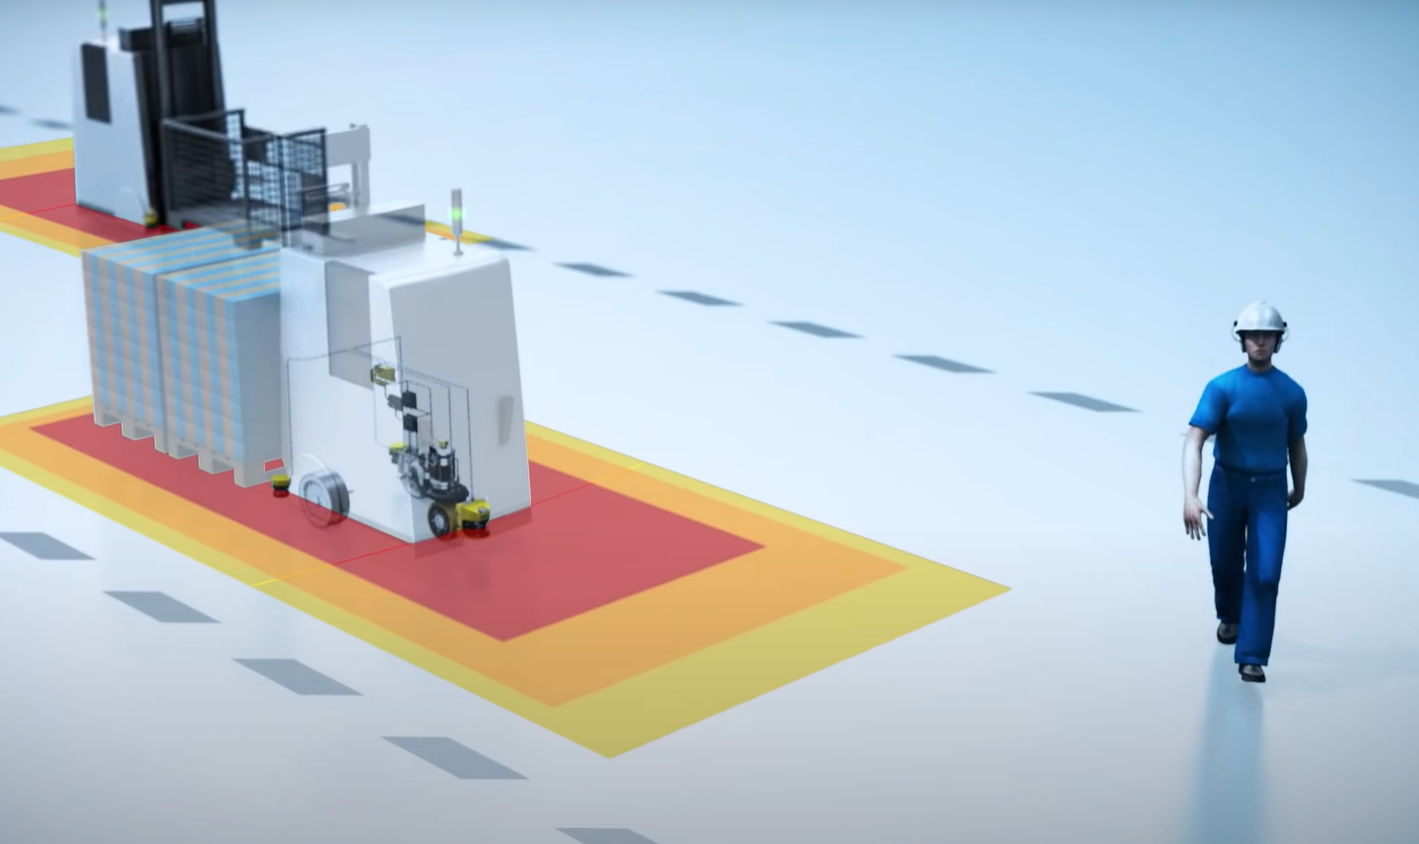
\includegraphics[width=(\textwidth)/2]{images/AGV_Show.png}
    \caption{AGV Simualtion}
    \label{fig:AGV}
\end{figure}
Die vorliegende Problemstellung bezieht sich auf die Integration in das Dynamic Simulation Model (DSM). Das Hauptziel besteht darin, eine realistische Umgebung zu schaffen, in der Szenarien aufgebaut und Sensorinformationen an den gRPC-Server übertragen werden können. Aktuell fehlt eine Simulation, die Gefahrensituationen für Tests und Validierungen ermöglicht. So sollen Testdaten generiert werden, die sich aus 2D LiDAR Sensordaten, der Geschwindigkeit des AGVs zusammensetzten. Mit den Testdaten können Algorithmen zur Schutzfeld Berechnung entwickelt werden.
Die in der Simulation getesteten Algorithmen im weiteren Entwicklung auch in realen Szenarien erprobt werden. Dies bietet erstmalig die Gelegenheit, die Leistungsfähigkeit der Sicherheitsalgorithmen zu erproben.
%Wo finde ich informationen zum DSM Projekt? Boris morgen fragen
%Was trage ich zu deisem Projekt bei?

%Spezifische Fragestellung: Formuliere deine Problemstellung als eine klare Frage. Diese Frage sollte präzise, klar und relevant sein. Vermeide vage oder mehrdeutige Formulierungen.


%Bedeutung und Relevanz Betone die Bedeutung deiner Problemstellung. Warum ist es wichtig, diese Frage zu beantworten oder dieses Problem zu lösen? Welche Auswirkungen könnte die Antwort haben?


%Abgrenzung und Kontext: Kläre den Rahmen deiner Problemstellung. Welche Aspekte deines Themas wirst du behandeln und welche wirst du bewusst außer Acht lassen? Definiere den Kontext, in dem deine Fragestellung relevant ist.


\section{Zielsetzung}
\begin{figure}[htp]
    \centering
    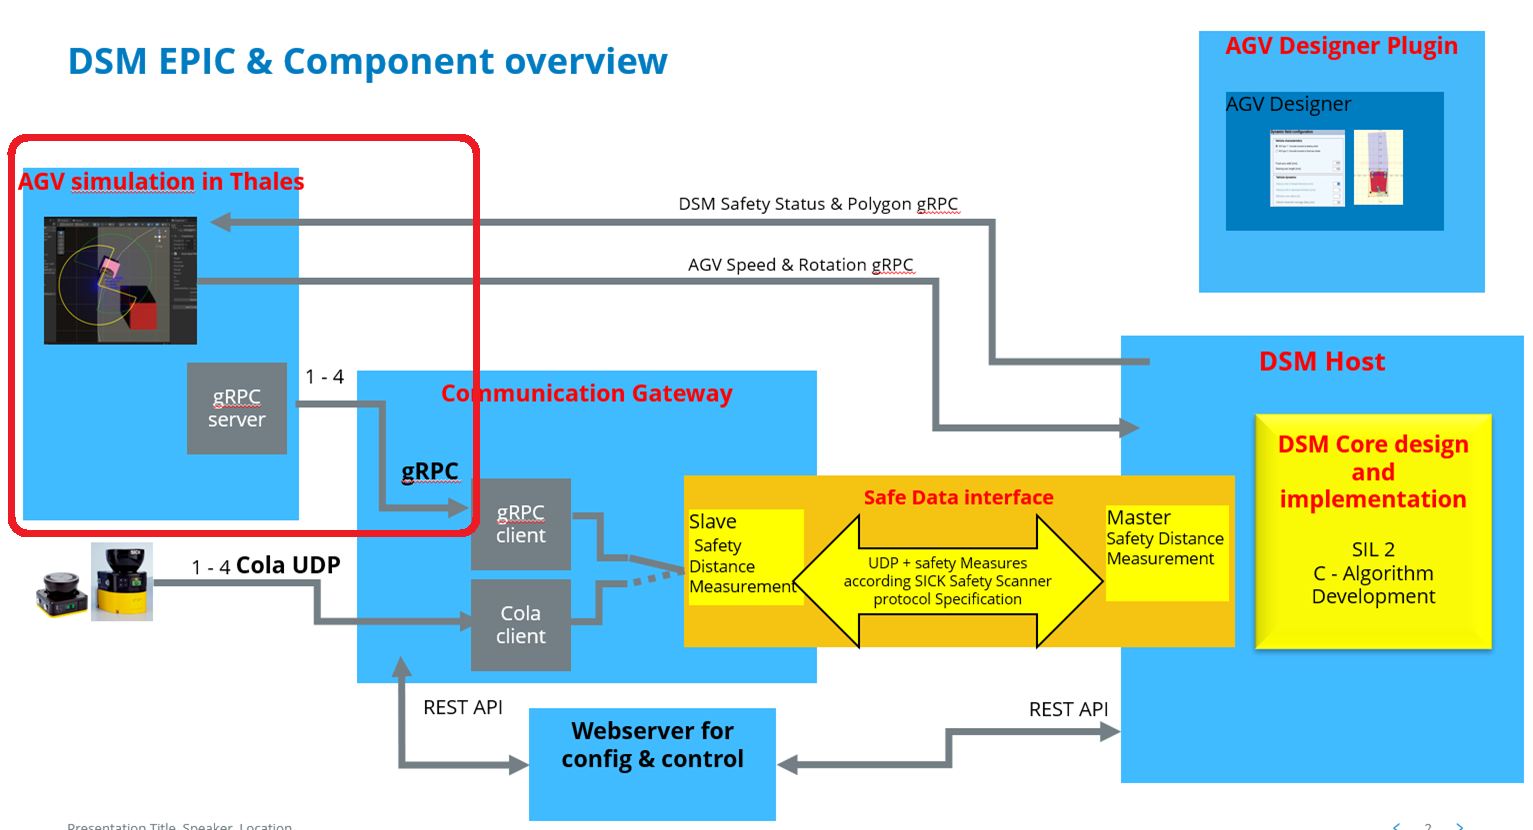
\includegraphics[width=(\textwidth)]{images/AGV_Overview.png}
    \caption{DSM EPIC \& Component overview}
    \label{fig:DSMoverview}
\end{figure}
%Die Zielsetzung beschreibt das übergeordnete Ziel deiner Arbeit. Sie verdeutlicht, was du mit deiner Forschung erreichen möchtest.
Die Projektarbeit hat als Ziel den rot markierten Bereich umzusetzen. Mit den erzeugten Daten sollen sollen im DSM Host die Sicherheitsalgorithmen entwickelt werden. Diese Entwicklung wird kein Teil dieser Projektarbeit.\\

Das Hauptziel dieser Arbeit besteht darin, die grundlegende Funktionalität eines Forschungsprojekts zur Entwicklung autonomer fahrerloser Fahrzeuge (AGVs) sicherzustellen und eine solide Grundlage für die weitere Entwicklung zu schaffen. Dazu werden mehrere Schlüsselaufgaben verfolgt.\\

Zunächst liegt der Fokus auf der Implementierung einer funktionsfähigen Schnittstelle zwischen dem gRPC-Server und dem Client, um die bidirektionale Übertragung von Daten zu ermöglichen. Ziel ist es, Thales Sensordaten von 4 Sensoren über den gRPC-Server abzurufen.\\

Eine weitere Schlüsselaufgaben ist es eine Schnittstelle zu implementieren um andere relevante Parameter wie den Lenkwinkel oder die Geschwindigkeit eines zukünftig erstellten AGVs übertragen zu können.\\

%Konkretheit: Formuliere deine Zielsetzung so konkret wie möglich. Vermeide allgemeine Formulierungen, die mehrdeutig sind.
%Messbarkeit: Stelle sicher, dass dein Ziel messbar ist. Das bedeutet, dass du später überprüfen können solltest, ob du es erreicht hast.
%Realistisch: Deine Zielsetzung sollte realistisch sein und in einem angemessenen Rahmen erreichbar sein.
%Relevanz: Betone, warum dein Ziel wichtig ist und welche Bedeutung es für die Forschung oder die Praxis hat.


%\section{Fragestellung}
%Die Forschungsfrage konkretisiert deine Zielsetzung und gibt die Richtung für deine Untersuchung vor. Sie sollte präzise, klar und offen genug sein, um die Möglichkeit zur Forschung zu bieten.
%Klarheit: Formuliere die Forschungsfrage klar und verständlich. Vermeide komplexe Satzstrukturen.
%Ein Frageaspekt: Fokussiere auf einen bestimmten Aspekt des Themas. Eine zu breite Fragestellung kann zu unübersichtlichen Ergebnissen führen.
%Beantwortbarkeit: Stelle sicher, dass deine Forschungsfrage durch deine Forschungsmethoden und Daten beantwortbar ist.

%Wie kann ein AGV in Unity in erstellt werden und dessen Meschanische Daten über gRPC mit der Ausenwelt geteilt werden und auch Daten erhalten? 